\documentclass{standalone}
\usepackage{tikz}

\begin{document}

%x description="draw a slice"
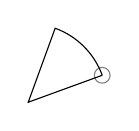
\begin{tikzpicture}
	\draw[gray] (0,0) circle[radius=0.1];
%x step={
\draw
	(0,0) arc [radius=1, start angle=20, delta angle=50] 
	% or 
	(0,0) arc [radius=1, start angle=20, end angle=70] % ignores delta angle
	% or
	(0,0) arc (20:70:1) % (start:end:radius)

	-- ++(70:-1) % polar coordinates (angle:distance)
	-- ++(20:1);
%x }
\end{tikzpicture}

\end{document}
